\chapter{Konzeption des Wissensquiz}
Konzeptionell stützt sich das 
\section{Analyse der vorhandenen Schulungsunterlagen}
\section{Erstellung und Aufbau des Fragenkatalogs}
\section{Darlegung des Prüf- und Freigabeprozesses}
% Gegenstand der Arbeitspaketeplanung ist die Struktur von Projekten hinsichtlich ihrer Komplexität.
% \footcite[Vgl.][128]{kusterHandbuchProjektmanagementAgil2022}
% Dies geschieht durch die Unterteilung des Projektes in kleinere Einheiten sowie durch die Erstellung eines Projektstrukturplans.
% Oftmals wird dieser einschließlich seiner Meilensteine auf Arbeitspaketebene aufgeteilt und somit für Projektmitarbeiter editierbar gemacht.
% \footcite[Vgl.][121]{panagosToolsUndMassnahmen2019}
% Dies ist vergleichbar mit einer umgekehrten Baumstruktur, bei welcher im oberen Bereich der jeweilige Meilenstein dargestellt ist und die Blätter die
% zugehörigen Arbeitspakete repräsentieren.
% \footcite[Vgl.][29]{kusay-merkleAgilesProjektmanagementIm2018}
% Im unteren Bereich sind schlussendlich die unteilbaren Arbeitspakete zu finden. In der Theorie können diese jedoch auf einer beliebigen Ebene liegen.
% \footcite[Vgl.][73]{gadatschGrundkursITProjektcontrollingGrundlagen2008}
% Das Finden von Arbeitspaketen findet hierbei ausgehend von der unteren Ebene statt.
% Diese eignet sich insbesondere für Projektvorhaben, welchen eine geringere Erfahrung mit dem zu behandelnden Themengebiet zugrunde liegt.
% Hierbei werden alle Tätigkeiten als Team zusammengeführt und anschließend Meilensteine mit den darunterliegenden Arbeitspaketen
% definiert (siehe Abb. \ref{abb:psp}).
% \footcite[Vgl.][133]{kusterHandbuchProjektmanagementAgil2022}
% \begin{figure}[H]
%     \centering
%     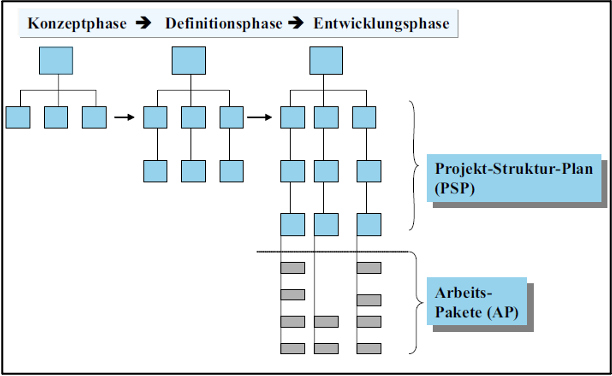
\includegraphics[width=0.47\linewidth]{graphics/psp.png}
%     \caption{Zuordnung von Arbeitspaketen innerhalb der Projektstrukturplanung.}\label{abb:psp}
% \end{figure}
% \section{Arbeitspaketebeschreibung und Aufwandsschätzung}
% Bestandteile bei der Defintion von Arbeitspaketen sind die Leistungsbeschreibung, die jeweils verantwortliche Person
% sowie die zugeordneten Ressourcen.
% \footcite[Vgl.][73]{gadatschGrundkursITProjektcontrollingGrundlagen2008}
% Zusätzlich können untergeordnete Aufgabenpakete mit entsprechenden Zeitangaben erstellt werden.
% \footcite[Vgl.][74]{gadatschGrundkursITProjektcontrollingGrundlagen2008}
% Als Ergebnis muss denoch schlussendlich ein minimal funktionsfähiges Produkt (in der Literatur: „\ac{MVP}“)
% vorliegen, welches im Sinne des Wasserfall-Modells in die nächste Phase übernommen werden kann.
% \footcite[Vgl.][52]{panagosToolsUndMassnahmen2019}
% Als weitere Anforderung an die Arbeitspakete soll beim vorliegenden Projekt dafür gesorgt sein, dass die Ausführung
% von einer einzelnen Person in einem angemessenen zeitlichen Rahmen bewältigt werden kann.
% In Projekten, welche unter wirtschaftlichen Rahmenbedingungen stattfinden, werden für die Schätzung des Zeitbedarfs
% der einzelnen Projektaktivitäten häufig \ac{PM} benutzt, bei welchen allerdings Vollzeitmitarbeiter als Grundlage
% angesehen werden.
% \footcite[Vgl.][74]{gadatschGrundkursITProjektcontrollingGrundlagen2008}
% Da dieser Umstand bei einem Hochschulprojekt nicht gegeben ist, wird daher mit keiner konkret geschätzten Zeit
% gearbeitet. Es wird hier nach interner Absprache zwischen dem Projektteam lediglich eine Abgabefrist für
% Arbeitspakete gesetzt, welche für alle am Projekt beteiligten Personen einzuhalten ist. Weitere Informationen
% hierzu sind in \textit{Kapitel 6} zu finden.
% \section{Backlog und Akzeptanzkriterien für Arbeitspakete}
% Das Backlog stellt eine Liste der gewünschten Arbeiten dar.
% \footcite[Vgl.][362]{kusay-merkleAgilesProjektmanagementIm2018}
% Diese noch zu erledigenden Aufgaben können dort bis zur abschließenden Nutzung gesammelt und aufbereitet werden.
% \footcite[Vgl.][362]{kusay-merkleAgilesProjektmanagementIm2018}
% Ferner werden die Arbeitspakete hierbei den großen Meilensteinen (in der Literatur: „Epics“) zugeordnet.
% Als Werkzeug für diese Arbeitspakete- und Zeitplanung kommt das Programm „Jira Software“ zum Einsatz.
% Es ist für kleine Projekte kostenlos nutzbar und enthält Funktionen für die Nachvollziehbarkeit von Aufgaben
% und Fehlern sowie für die Verwaltung von Projekten.
% \footcite[Vgl.][3]{ortuMeasuringUnderstandingEffectiveness2015}
% Als vorteilhaft bei der Nutzung von Jira erweist sich der grundflexible Charakter der Software, welcher
% es dem Projektteam unter anderem ermöglicht, Teilinkremente mit hoher Produktivität auszuliefern, das Backlog zu verwalten
% sowie den Fortschritt des Projekts visuell darzustellen.
% \footcite[Vgl.][3]{ortuMeasuringUnderstandingEffectiveness2015}
% Die aktuellen Meilensteine im Backlog sind folgende:
% \begin{enumerate}
%     \item Ausarbeitung der Projektkonzeption
%     \item Präsentation am Anfang des sechsten Semesters
%     \item Interviews mit Leitfaden
%     \item Wissenschaftliche Ausarbeitung im sechsten Semester
%     \item Prototyp im sechsten Semester
%     \item Ergebnispräsentation am Ende des sechsten Semesters
% \end{enumerate}
% Im Backlog werden schließlich für die einzelnen Arbeitspakete der Meilensteine Kriterien erstellt, anhand derer
% erkenntlich wird, ob das jeweilige Objekt den Anforderungen entsprechend umgesetzt worden ist.
% \footcite[Vgl.][46]{kusay-merkleAgilesProjektmanagementIm2018}
% Vor der Fertigstellung eines Arbeitspakets müssen alle vorher definierten Akzeptanzkriterien erfüllt sein.
% \footcite[Vgl.][154]{kusterHandbuchProjektmanagementAgil2022}